%! TeX program = lualatex
\documentclass[12pt,a4paper]{instrukcja}

\begin{document}

% \begin{center}
	\vspace*{2cm}

 	\hrulefill
	
	\vspace{0.7cm}
	

		\textbf{\textsc{{\Huge{Obrzędy Wielkiego Tygodnia}}\\\bigskip{\large wg OHS 1955-1962}}}
	
	\vspace{0.5cm}
	
	\hrulefill

	\vspace{\fill}	

	 {\large \textbf{Użyte oznaczenia:}} \\
	
	 \vspace{0.1\textwidth}
	 
	 {\large\centering
	   \begin{itemize}[leftmargin=.43\linewidth,rightmargin=.35\linewidth,label=]
	    \item \ii~ -- celebrans 
	    \item \dd~ -- diakon 
	    \item \ss~ -- subdiakon
 	    \item \cc~ -- ceremoniarze 
	    \item \aa~ -- akolici 
	    \item \tt~ -- turyferarz 
	    \item \ding{63} -- krzyż procesyjny
	    \item \oo -- ombrelino
	  \end{itemize}
	 }
	
	\vspace{5cm}	
	
	\hrulefill
	
	{\footnotesize Pierwsza edycja -- 9 kwietnia 2017\\
	Druga edycja -- 8 kwietnia 2019 \\
	Wszelkie zastrzeżenia proszę kierować do autora na adres: \texttt{michal96.96@gmail.com}}

	\newpage
\end{center}

	

\thispagestyle{empty}

\pagestyle{plain}

% \tableofcontents

% \newpage

\chapter{Niedzila Palmowa}

\section{Przygotowanie do obrzędów}
		
		\subsection{W zakrystii}
		
			\begin{itemize}
   				\item dla \ii: humerał, alba z koronką, cingulum białe, stuła i kapa: {\color{red}czerwone},
				\item dla \dd: humerał, alba z koronką, cingulum białe, stuła i dalmatyka: {\color{red}czerwone},
				\item dla \ss: humerał, alba z koronką, cingulum białe, tunicela {\color{red}czerwona},
				\item dla \ding{63}: tunicela {\color{red}czerwona},
				\item akolitki,
				\item kadzielnica z łódką, 
			\end{itemize}
		
		\subsection{Na kredensji w kościele}
		
			\begin{itemize}
				\item kielich do Mszy św. z wszystkimi paramentami barwy  {\color{violet}fioletowej} (w tym welon naramienny dla \ss),
				\item tacka z ampułkami i ręcznikiem do Mszy św.,
				\item dzwonek,
				\item 2 pateny,
				\item 2 świeczki \textit{Sanctusowe},
%				\item księga OHS, 
				\item lekcjonarz,
				\item teksty pasji z nutami (po polsku),
			\end{itemize}
		
%			W miarę możliwości kielich i paramenta {\color{violet}fioletowe} do chwili zakończenia procesji powinny być zakryte {\color{red}czerwoną} zasłoną.
			
		\subsection{Na ołtarzu polowym}
			
			\begin{itemize}
				\item krzyż,
				\item 6 świec z osłonkami,
				\item księga OHS ubrana we {\color{violet}fioletową} okładkę,
				\item pulpit albo poduszka na OHS,
			\end{itemize}
		
		\subsection{Na kredensji na dworze}
			
			\begin{itemize}
				\item naczynie z wodą święconą i kropidło,
				\item ewangeliarz ubrany w {\color{red}czerwoną} okładkę,
%				\item lekcjonarz dla diakona do śpiewania,
				\item mydło, miska i dzbanek z wodą do umycia rąk celebransa po rozdaniu palm,
				\item ręcznik,
%				\item teksty do recytowania podczas procesji,
				\item miejsce na akolitki,
				\item miejsce na birety,
			\end{itemize}
		
		\subsection{Na Sedilli w kościele}
		
			\begin{itemize}
				\item dla \ii~ manipularz, stuła i ornat – {\color{violet}fioletowe},
				\item dla \dd~ manipularz, stuła i dalmatyka – {\color{violet}fioletowe},
				\item dla \ss~ manipularz i tunicela – {\color{violet}fioletowe},
			\end{itemize}
	
		\subsection{Po stronie ewangelii}
			
			\begin{itemize}
				\item trzy wysokie pulpity bez nakrycia do śpiewania pasji \footnote{ustawione na północ chyba że nie uda się zorganizować mikrofonów},
				\item przynajmniej jeden mikrofon.
			\end{itemize}

\section{Procesja wejścia}

\begin{itemize*}
	\item Standardowa procesja wejścia. Jeśli jest \ding{63}, idzie on między
	      \aa~. \tt~ niesie trybularz i łódkę. \cc2 idzie w parze z \tt. \ii~ ubrany
	      jest w fioletową kapę.
	\item Liturgia może rozpocząć się od kazania (jak w 2019 roku).
\end{itemize*}

	\section{Msza Święta - ważniejsze zmiany}
		\begin{itemize}
		 \item wszyscy odkładają palmy
		 \item nie odmawia się modlitw u stopni
		 \item bezpośrednio po przyklęknięciu następuje ucałowanie ołtarza i nałożenie kadzidła
		 \item po odmówieniu \textit{Introitu} i \textit{Kyrie} $\mathcal{I}$ i $\mathcal{D}$ oraz $\mathcal{S}$ krótką drogą schodzą do sedilii
		 \item podczas lekcji na słowa \textit{in nomine Iesu omne genu flectatur} wszyscy przyklękają
		 \item procesja przed Ewanglią, jak i funkcje tworzących ich ministrantów pozostają (prawie) bez zmian względem Mszy śpiewanej (za wyjątkiem nietrzymania w jej czasie paramentów litrugicznych); więcej patrz \hyperref[E]{Dodatek}
		 \item chór podczas Ewangelii wykonuje skłony w kierunku krzyża ołtarzowego, a śpiewacy ``przed siebie``
		 \item po przyjęciu przez $\mathcal{I}$ Komunii Św. i wyciągnięciu puszki z tabernakulum $\mathcal{D}$ \textbf{sam} odmawia \textit{Confiteor}, po którym nastepuje \textit{Misereatur} -- \textbf{wszyscy} są w tym czasie pochyleni. Prostujemy się dopiero na \textit{Indulgenciam}
		 \item nie ma ostatniej Ewangelii
		
		\end{itemize}

\section{Dodatek}
\label{sec:dodatek_palm}

\subsection[Losy subdiakona krucyfera]{Losy subdiakona krucyfera \protect \footnote{Wymagany level -- obłuczony kleryk}}
\begin{itemize}
      \item subdiakon krucyfer ( \ding{63} ), ubrany w albę, cingulum i czerwoną
            tunicellę
      \item nie odbiera palmy od \ii
      \item po skończonej procesji idzie do kaplicy zimowej, gdzie ściąga westymenta
            subdiakona, zakłada komżę, bierze biret i przechodzi do chóru
\end{itemize}

\subsection{Procesja do Ewangelii - dla zaawansowanych}

\subsubsection*{\textbf{Celebrans z subdiakonem i ceremoniarzem }}
\begin{itemize}
      \item kiedy skończy się śpiew \textit{Graduału} i \textit{Traktusa}, \ii~ wraz
            z \ss~ i \cc1 podchodzą do ołtarza - przyklękają
      \item \ii~ wchodzi na najwyższy stopień i odmawia modlitwę \textit{Munda cor}
      \item \ss~ w tym czasie przenosi mszał
      \item \ss~ przechodzi ze Mszałem na stronę Ewangelii i pozostaje przy nim
            asystując \ii~ przy kartkach
      \item \cc1, \tt, \aa1, \aa2 \textbf{nie} ustawiają się jak na Mszy
            śpiewanej (zostają na swoich bazach) \footnote{Ceremoniał o.
                  Małaczyńskiego, str. 65, pkt. 47(dla rytu uroczystego): „Jeżeli Męka
                  Pańska nie jest śpiewana celebrans pod koniec traktusa odmawia
                  \textit{Munda cor} i czyta Mękę Pańską po stronie Ewangelii.
                  Równocześnie należy ją odczytać wiernym  po polsku."}
      \item \ii~ po przeczytaniu Pasji nie schodzi do sedilli tylko idzie na
            stronę lekcji i obraca się w kierunku śpiewanej pasji; \ss~ stoi na
            swoim stopniu (\textit{in plano}) po stronie lekcji odwrócony w
            stronę pasji, mogą wziąć palmy
\end{itemize}

\subsubsection*{\textbf{Diakon i śpiewacy}}
\begin{itemize}
      \item \dd, przy pomocy \cc2, zdejmuje dalmatykę i manipularz
      \item \dd, od \cc2, otrzymuje księgę z tekstem Pasji
      \item \cc2 prowadzi \dd~ do ambony, \eighthnote1 i \eighthnote2 czekają na
            miejscu; śpiew pasji wykonywany jest po stronie ewangelii przed
            balaskami
      \item wszystkie skłony podczas Pasji wykonujemy w stronę
            ewangeliarza/lekcjonarza (nie w stronę Mszału),
      \item po skończonej Pasji \dd~ i \cc2 przyklękają na środku, po czym \cc2
            prowadzi \dd~ do sedilli i pomaga mu założyć dalmatykę i manipularz
      \item \dd~ zajmuje swoje miejsce za \ii~ i przyklęka --
            \ii~ rozpoczyna \textit{Credo}
\end{itemize}

\newpage

% \chapter{Niedzila Palmowa}

\section{Przygotowanie do obrzędów}
		
		\subsection{W zakrystii}
		
			\begin{itemize}
   				\item dla \ii: humerał, alba z koronką, cingulum białe, stuła i kapa: {\color{red}czerwone},
				\item dla \dd: humerał, alba z koronką, cingulum białe, stuła i dalmatyka: {\color{red}czerwone},
				\item dla \ss: humerał, alba z koronką, cingulum białe, tunicela {\color{red}czerwona},
				\item dla \ding{63}: tunicela {\color{red}czerwona},
				\item akolitki,
				\item kadzielnica z łódką, 
			\end{itemize}
		
		\subsection{Na kredensji w kościele}
		
			\begin{itemize}
				\item kielich do Mszy św. z wszystkimi paramentami barwy  {\color{violet}fioletowej} (w tym welon naramienny dla \ss),
				\item tacka z ampułkami i ręcznikiem do Mszy św.,
				\item dzwonek,
				\item 2 pateny,
				\item 2 świeczki \textit{Sanctusowe},
%				\item księga OHS, 
				\item lekcjonarz,
				\item teksty pasji z nutami (po polsku),
			\end{itemize}
		
%			W miarę możliwości kielich i paramenta {\color{violet}fioletowe} do chwili zakończenia procesji powinny być zakryte {\color{red}czerwoną} zasłoną.
			
		\subsection{Na ołtarzu polowym}
			
			\begin{itemize}
				\item krzyż,
				\item 6 świec z osłonkami,
				\item księga OHS ubrana we {\color{violet}fioletową} okładkę,
				\item pulpit albo poduszka na OHS,
			\end{itemize}
		
		\subsection{Na kredensji na dworze}
			
			\begin{itemize}
				\item naczynie z wodą święconą i kropidło,
				\item ewangeliarz ubrany w {\color{red}czerwoną} okładkę,
%				\item lekcjonarz dla diakona do śpiewania,
				\item mydło, miska i dzbanek z wodą do umycia rąk celebransa po rozdaniu palm,
				\item ręcznik,
%				\item teksty do recytowania podczas procesji,
				\item miejsce na akolitki,
				\item miejsce na birety,
			\end{itemize}
		
		\subsection{Na Sedilli w kościele}
		
			\begin{itemize}
				\item dla \ii~ manipularz, stuła i ornat – {\color{violet}fioletowe},
				\item dla \dd~ manipularz, stuła i dalmatyka – {\color{violet}fioletowe},
				\item dla \ss~ manipularz i tunicela – {\color{violet}fioletowe},
			\end{itemize}
	
		\subsection{Po stronie ewangelii}
			
			\begin{itemize}
				\item trzy wysokie pulpity bez nakrycia do śpiewania pasji \footnote{ustawione na północ chyba że nie uda się zorganizować mikrofonów},
				\item przynajmniej jeden mikrofon.
			\end{itemize}

% \section{Procesja wejścia}

\begin{itemize*}
	\item Standardowa procesja wejścia. Jeśli jest \ding{63}, idzie on między
	      \aa~. \tt~ niesie trybularz i łódkę. \cc2 idzie w parze z \tt. \ii~ ubrany
	      jest w fioletową kapę.
	\item Liturgia może rozpocząć się od kazania (jak w 2019 roku).
\end{itemize*}

% \section{Uroczyste modły}

\begin{itemize}
      \item \zz~ przynosi z zakrystii czarną kapę
      \item \ii~ zakłada czarną kapę przy pomocy \cc1 i \cc2
      \item  w tym czasie \aa1 oraz \aa2 rozkładają na ołtarzu jeden obrus oraz
            ustawiają na środku pulpit z mszałem oraz kartką z wezwaniem
            modlitwy powszechnej za żydów, potem wracają na swoje miejsca przy
            kredencji
      \item  \ii~ wraz z \cc1 i \cc2 przytrzymującymi brzegi kapy podchodzi
            przed ołtarz, wykonują ukłon i wchodzą na stopnie
      \item  \ii~ całuje mensę ołtarzową i rozpoczyna śpiew modlitw
      \item  na wezwanie \textit{Flectamus genua} wszyscy klękają, na
            \textit{Levate} – wstają
      \item  po zakończeniu modlitw \ii~, \cc1 i \cc2 skłaniają głowy i wracają
            do sedilli krótką drogą, \cc1 i \cc2 trzymają kapę
      \item \tt1 zabiera mszał wraz ze stojakiem z ołtarza
      \item  \ii~ zdejmuje kapę, którą Z odnosi do zakrystii
\end{itemize}

% \section{Dodatek}
\label{sec:dodatek_palm}

\subsection[Losy subdiakona krucyfera]{Losy subdiakona krucyfera \protect \footnote{Wymagany level -- obłuczony kleryk}}
\begin{itemize}
      \item subdiakon krucyfer ( \ding{63} ), ubrany w albę, cingulum i czerwoną
            tunicellę
      \item nie odbiera palmy od \ii
      \item po skończonej procesji idzie do kaplicy zimowej, gdzie ściąga westymenta
            subdiakona, zakłada komżę, bierze biret i przechodzi do chóru
\end{itemize}

\subsection{Procesja do Ewangelii - dla zaawansowanych}

\subsubsection*{\textbf{Celebrans z subdiakonem i ceremoniarzem }}
\begin{itemize}
      \item kiedy skończy się śpiew \textit{Graduału} i \textit{Traktusa}, \ii~ wraz
            z \ss~ i \cc1 podchodzą do ołtarza - przyklękają
      \item \ii~ wchodzi na najwyższy stopień i odmawia modlitwę \textit{Munda cor}
      \item \ss~ w tym czasie przenosi mszał
      \item \ss~ przechodzi ze Mszałem na stronę Ewangelii i pozostaje przy nim
            asystując \ii~ przy kartkach
      \item \cc1, \tt, \aa1, \aa2 \textbf{nie} ustawiają się jak na Mszy
            śpiewanej (zostają na swoich bazach) \footnote{Ceremoniał o.
                  Małaczyńskiego, str. 65, pkt. 47(dla rytu uroczystego): „Jeżeli Męka
                  Pańska nie jest śpiewana celebrans pod koniec traktusa odmawia
                  \textit{Munda cor} i czyta Mękę Pańską po stronie Ewangelii.
                  Równocześnie należy ją odczytać wiernym  po polsku."}
      \item \ii~ po przeczytaniu Pasji nie schodzi do sedilli tylko idzie na
            stronę lekcji i obraca się w kierunku śpiewanej pasji; \ss~ stoi na
            swoim stopniu (\textit{in plano}) po stronie lekcji odwrócony w
            stronę pasji, mogą wziąć palmy
\end{itemize}

\subsubsection*{\textbf{Diakon i śpiewacy}}
\begin{itemize}
      \item \dd, przy pomocy \cc2, zdejmuje dalmatykę i manipularz
      \item \dd, od \cc2, otrzymuje księgę z tekstem Pasji
      \item \cc2 prowadzi \dd~ do ambony, \eighthnote1 i \eighthnote2 czekają na
            miejscu; śpiew pasji wykonywany jest po stronie ewangelii przed
            balaskami
      \item wszystkie skłony podczas Pasji wykonujemy w stronę
            ewangeliarza/lekcjonarza (nie w stronę Mszału),
      \item po skończonej Pasji \dd~ i \cc2 przyklękają na środku, po czym \cc2
            prowadzi \dd~ do sedilli i pomaga mu założyć dalmatykę i manipularz
      \item \dd~ zajmuje swoje miejsce za \ii~ i przyklęka --
            \ii~ rozpoczyna \textit{Credo}
\end{itemize}

% \section{Dodatek}

\subsection{Przebieg poświęcenia wody}
\label{sec:woda}
\begin{enumerate}
      \item \textit{Dominus Vobiscum} i Oracja 0. (przed wejściem)
            \smallfont{(złożone ręce)}
      \item \textit{Dominus Vobiscum} i Oracja 1. \smallfont{(złożone ręce)}
      \item Prefacja do słów \textit{Sumat unigeniti tui gratiam de Spiritu
                  Sancto}
      \item Celebrans kreśli znak krzyża
            \textcolor{red}{\raisebox{-1mm}{\scalebox{1.5}{\ding{64}}}} na
            wodzie
      \item Wyciera ręce
      \item Kontynuuje modlitwę
      \item Na \textit{Sit haec} kładzie rękę na powierzchni wody
      \item Wyciera rękę
      \item Kreśli znaki krzyża
            \textcolor{red}{\raisebox{-1mm}{\scalebox{1.5}{\ding{64}}}}
            nad wodą na słowa \textit{Per Deum vivum \dots}
            \vspace*{-11pt}
      \item Wylewa wodę na cztery strony świata po słowach \textit{... super te
                  ferebatur} ~~~
            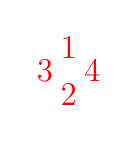
\begin{tikzpicture}[scale=0.3, baseline=-1mm, thick]
                  \draw[color=red] (10mm,0) node {\large 4};
                  \draw[color=red] (-10mm,0) node {\large 3};
                  \draw[color=red] (0,10mm) node {\large 1};
                  \draw[color=red] (0,-10mm) node {\large 2};
            \end{tikzpicture}
            \vspace*{-7pt}
      \item Kreśli znak krzyża nad wodą na \textit{Benedico te}
      \item Po zmianie głosu na \textit{recto tono} na słowa \textit{tu benignus
                  aspira} trzy razy dmucha do wody na kształt krzyża
      \item W tym czasie ceremoniarz podaje Paschał
      \item Na słowa \textit{Descendad in hanc} trzy razy wkłada Paschał do wody
            i śpiewa \footnote{Wkłada Paschał coraz głębiej}
      \item \ii~ trzy razy dmucha do wody w kształcie litery
            \textcolor{red}{\raisebox{-1mm}{\Large ${\Psi}$}} i kontynuuje
            \textit{Totamque ... effectu}
      \item Wyciągamy Paschał z wody i kończymy święcenie wody (\textit{... per
                  ignem.})
      \item Po wyjęciu paschału nabiera się wody do pokropienia
      \item Następnie \cc1 przynosi do chrzcielnicy tackę z olejami świętymi i
            wręcza \ii~ (z pocałunkiem) odpowiednie ampułki. \ii, wypowiadając
            słowa przepisane w księdze po kolei:
            \begin{itemize}
                  \item wlewa olej katechumenów
                  \item wlewa krzyżmo
                  \item wlewa oba
            \end{itemize}
      \item Następnie miesza wodę ręką lub przy pomocy łyżeczki
      \item Później myje i wyciera ręce \footnote{W razie potrzeby wykorzystuje
                  sól, watę i miękisz chleba, które później należy spalić. Wodę
                  z tej ablucji wlewa
                  się do sacrarium.}
\end{enumerate}

\subsection{Bierzmowanie}
\label{sec:bierz}
\begin{itemize}
      \item księgę z modlitwami trzyma \cc1, a \cc2 podtrzymuje kapę jeśli
            trzeba; \aa1 i \aa2 stoją z boku przy kredencji
      \item \ii~ odmawia modlitwę zwracając się do kandydatów \textit{Spiritus
                  Sanctus superveniat\dots}
      \item \ii~ czyni znak Krzyża Świetego mówiąc \textit{Adjutorium
                  nostrum...} a następnie kontynuowany jest krótki dialog
      \item \ii~ wyciąga ręce nad przystępującymi do bierzmowania i mówi
            \textit{Oremus. Omnipotens sempiterne Deus,...}
      \item przystępujący do sakramentu klęka przed \ii. Świadek kładzie rękę na
            prawym ramieniu bierzmowanego.
      \item \aa1 podchodzi do \ii~ z Krzyżmem Świętem
      \item \ii~ kładzie prawą rękę na głowie bierzmowanego i palcem umoczonym w
            Krzyżmie Świętym robi znak krzyż a na czole, mówiąc \textit{Signo te
                  signo...}
      \item \ii~ uderza lekko w policzek bierzmowanego, mówiąc \textit{Pax tecum}
      \item kandydat wraca na swoje wcześniejsze miejsce i stoi
      \item \aa1 odbiera Krzyżmo, a \aa2 podchodzi z czymś do wytarcia palców
            \footnote{najpewniej wata}; później wracają do kredencji
      \item gdy \ii~ namaści wszystkich kandydatów, śpiewa się antyfonę
            \textit{Confirma hoc, Deus\dots}
      \item powtarza się antyfonę, a następnie \ii~ zwrócony do ołtarza śpiewa
            \textit{Ostende nobis, Domine,...}, a następnie \textit{Oremus.
                  Deus, qui Apostolis tuis\dots}
      \item \ii~ mówi \textit{Ecce sic benedicetur omnis homo, qui timet Dominum}
      \item na końcu \ii~ błogosławi bierzmowanych
            \textit{Bene} + \textit{dicat vos Dominus ex Sion...}
\end{itemize}

\color{red}

\section{Uwagi}
\begin{itemize}
      \item można zrobić jakieś święcenie ognia przed proroctwami tak aby ludzie
            oświetlali kościół i mieć jakąś namiastkę Wigilii Paschalnej
      \item na poświęcenie wody ludzie \textbf{muszą mieć zapalne świece}
      \item zapytać księdza czy będzie aspersja (czy to humanitarne?)
      \item ziomek do chrztu musi siedzieć za kratą aż do ochrzczenia -- trzeba
            mu przygotować jakieś krzesło i klęcznik
      \item na chrzest dorosłego ksiądz ubiera kapę (patrz Nowowiejski)
\end{itemize}

% \newpage

% \chapter{Wielki Piątek}

\section{Przygotowanie do obrzędów}
    
        \subsection{Ołtarz główny}
        
            \begin{itemize}
                \item zupełnie ogołocony
                \item tabernakulum puste, obok kluczyk
                \item na tabernakulum podstawa pod krzyż
                \item na najwyższym stopniu jedna fioletowa poduszka do prostracji
                \item za ołtarzem odkryty krzyż procesyjny
            \end{itemize}
        
        \subsection{Kredencja}
        
            \begin{itemize}
                \item przykryta normalnie obrusem
                \item jeden obrus ołtarzowy
                \item pulpit pod mszał, razem z mszałem
                \item księga OHS
                \item pozostałe dwie fioletowe poduszki pod krzyż
                \item ręczniczek do wycierania krzyża
                \item fioletowa bursa z korporałem
                \item dwie pateny komunijne
                \item dwie świece sanctusowe
                \item vasculum i ręczniczek
                \item akolitki
                \item monstrancja
                \item welon do monstrancji
            \end{itemize}
        
        \subsection{Zakrystia/kaplica}
        
            \begin{itemize}
                \item czarna kapa
                \item fioletowy ornat ze stułą
                \item fioletowa kapa
                \item zasłonięty krzyż do adoracji
                \item 4 świeczniki z żółtymi świecami (i zapalniczka)
                \item biały welon naramienny
                \item dwa trybularze, jedna łódka
                \item ombrelino
            \end{itemize}
        
        \subsection{Inne}
        
            \begin{itemize}
                \item przy sedilli dodatkowe dwa miejsca dla ceremoniarzy (za akolitami)
                \item wysoki pulpit do śpiewu lekcji
                \item teksty Pasji do śpiewania
                \item dwie kołatki
                \item schodki
                \item fioletowa stuła dla ks. Ireneusza do Komunii
                \item świece na procesję dla ministrantów (z okapnikami, zapalniczki)
            \end{itemize}
        

% \section{Procesja wejścia}

\begin{itemize*}
	\item Standardowa procesja wejścia. Jeśli jest \ding{63}, idzie on między
	      \aa~. \tt~ niesie trybularz i łódkę. \cc2 idzie w parze z \tt. \ii~ ubrany
	      jest w fioletową kapę.
	\item Liturgia może rozpocząć się od kazania (jak w 2019 roku).
\end{itemize*}

% \section{Uroczyste modły}

\begin{itemize}
      \item \zz~ przynosi z zakrystii czarną kapę
      \item \ii~ zakłada czarną kapę przy pomocy \cc1 i \cc2
      \item  w tym czasie \aa1 oraz \aa2 rozkładają na ołtarzu jeden obrus oraz
            ustawiają na środku pulpit z mszałem oraz kartką z wezwaniem
            modlitwy powszechnej za żydów, potem wracają na swoje miejsca przy
            kredencji
      \item  \ii~ wraz z \cc1 i \cc2 przytrzymującymi brzegi kapy podchodzi
            przed ołtarz, wykonują ukłon i wchodzą na stopnie
      \item  \ii~ całuje mensę ołtarzową i rozpoczyna śpiew modlitw
      \item  na wezwanie \textit{Flectamus genua} wszyscy klękają, na
            \textit{Levate} – wstają
      \item  po zakończeniu modlitw \ii~, \cc1 i \cc2 skłaniają głowy i wracają
            do sedilli krótką drogą, \cc1 i \cc2 trzymają kapę
      \item \tt1 zabiera mszał wraz ze stojakiem z ołtarza
      \item  \ii~ zdejmuje kapę, którą Z odnosi do zakrystii
\end{itemize}

% \section{Dodatek}
\label{sec:dodatek_palm}

\subsection[Losy subdiakona krucyfera]{Losy subdiakona krucyfera \protect \footnote{Wymagany level -- obłuczony kleryk}}
\begin{itemize}
      \item subdiakon krucyfer ( \ding{63} ), ubrany w albę, cingulum i czerwoną
            tunicellę
      \item nie odbiera palmy od \ii
      \item po skończonej procesji idzie do kaplicy zimowej, gdzie ściąga westymenta
            subdiakona, zakłada komżę, bierze biret i przechodzi do chóru
\end{itemize}

\subsection{Procesja do Ewangelii - dla zaawansowanych}

\subsubsection*{\textbf{Celebrans z subdiakonem i ceremoniarzem }}
\begin{itemize}
      \item kiedy skończy się śpiew \textit{Graduału} i \textit{Traktusa}, \ii~ wraz
            z \ss~ i \cc1 podchodzą do ołtarza - przyklękają
      \item \ii~ wchodzi na najwyższy stopień i odmawia modlitwę \textit{Munda cor}
      \item \ss~ w tym czasie przenosi mszał
      \item \ss~ przechodzi ze Mszałem na stronę Ewangelii i pozostaje przy nim
            asystując \ii~ przy kartkach
      \item \cc1, \tt, \aa1, \aa2 \textbf{nie} ustawiają się jak na Mszy
            śpiewanej (zostają na swoich bazach) \footnote{Ceremoniał o.
                  Małaczyńskiego, str. 65, pkt. 47(dla rytu uroczystego): „Jeżeli Męka
                  Pańska nie jest śpiewana celebrans pod koniec traktusa odmawia
                  \textit{Munda cor} i czyta Mękę Pańską po stronie Ewangelii.
                  Równocześnie należy ją odczytać wiernym  po polsku."}
      \item \ii~ po przeczytaniu Pasji nie schodzi do sedilli tylko idzie na
            stronę lekcji i obraca się w kierunku śpiewanej pasji; \ss~ stoi na
            swoim stopniu (\textit{in plano}) po stronie lekcji odwrócony w
            stronę pasji, mogą wziąć palmy
\end{itemize}

\subsubsection*{\textbf{Diakon i śpiewacy}}
\begin{itemize}
      \item \dd, przy pomocy \cc2, zdejmuje dalmatykę i manipularz
      \item \dd, od \cc2, otrzymuje księgę z tekstem Pasji
      \item \cc2 prowadzi \dd~ do ambony, \eighthnote1 i \eighthnote2 czekają na
            miejscu; śpiew pasji wykonywany jest po stronie ewangelii przed
            balaskami
      \item wszystkie skłony podczas Pasji wykonujemy w stronę
            ewangeliarza/lekcjonarza (nie w stronę Mszału),
      \item po skończonej Pasji \dd~ i \cc2 przyklękają na środku, po czym \cc2
            prowadzi \dd~ do sedilli i pomaga mu założyć dalmatykę i manipularz
      \item \dd~ zajmuje swoje miejsce za \ii~ i przyklęka --
            \ii~ rozpoczyna \textit{Credo}
\end{itemize}

% \section{Dodatek}

\subsection{Przebieg poświęcenia wody}
\label{sec:woda}
\begin{enumerate}
      \item \textit{Dominus Vobiscum} i Oracja 0. (przed wejściem)
            \smallfont{(złożone ręce)}
      \item \textit{Dominus Vobiscum} i Oracja 1. \smallfont{(złożone ręce)}
      \item Prefacja do słów \textit{Sumat unigeniti tui gratiam de Spiritu
                  Sancto}
      \item Celebrans kreśli znak krzyża
            \textcolor{red}{\raisebox{-1mm}{\scalebox{1.5}{\ding{64}}}} na
            wodzie
      \item Wyciera ręce
      \item Kontynuuje modlitwę
      \item Na \textit{Sit haec} kładzie rękę na powierzchni wody
      \item Wyciera rękę
      \item Kreśli znaki krzyża
            \textcolor{red}{\raisebox{-1mm}{\scalebox{1.5}{\ding{64}}}}
            nad wodą na słowa \textit{Per Deum vivum \dots}
            \vspace*{-11pt}
      \item Wylewa wodę na cztery strony świata po słowach \textit{... super te
                  ferebatur} ~~~
            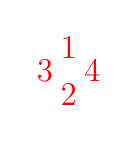
\begin{tikzpicture}[scale=0.3, baseline=-1mm, thick]
                  \draw[color=red] (10mm,0) node {\large 4};
                  \draw[color=red] (-10mm,0) node {\large 3};
                  \draw[color=red] (0,10mm) node {\large 1};
                  \draw[color=red] (0,-10mm) node {\large 2};
            \end{tikzpicture}
            \vspace*{-7pt}
      \item Kreśli znak krzyża nad wodą na \textit{Benedico te}
      \item Po zmianie głosu na \textit{recto tono} na słowa \textit{tu benignus
                  aspira} trzy razy dmucha do wody na kształt krzyża
      \item W tym czasie ceremoniarz podaje Paschał
      \item Na słowa \textit{Descendad in hanc} trzy razy wkłada Paschał do wody
            i śpiewa \footnote{Wkłada Paschał coraz głębiej}
      \item \ii~ trzy razy dmucha do wody w kształcie litery
            \textcolor{red}{\raisebox{-1mm}{\Large ${\Psi}$}} i kontynuuje
            \textit{Totamque ... effectu}
      \item Wyciągamy Paschał z wody i kończymy święcenie wody (\textit{... per
                  ignem.})
      \item Po wyjęciu paschału nabiera się wody do pokropienia
      \item Następnie \cc1 przynosi do chrzcielnicy tackę z olejami świętymi i
            wręcza \ii~ (z pocałunkiem) odpowiednie ampułki. \ii, wypowiadając
            słowa przepisane w księdze po kolei:
            \begin{itemize}
                  \item wlewa olej katechumenów
                  \item wlewa krzyżmo
                  \item wlewa oba
            \end{itemize}
      \item Następnie miesza wodę ręką lub przy pomocy łyżeczki
      \item Później myje i wyciera ręce \footnote{W razie potrzeby wykorzystuje
                  sól, watę i miękisz chleba, które później należy spalić. Wodę
                  z tej ablucji wlewa
                  się do sacrarium.}
\end{enumerate}

\subsection{Bierzmowanie}
\label{sec:bierz}
\begin{itemize}
      \item księgę z modlitwami trzyma \cc1, a \cc2 podtrzymuje kapę jeśli
            trzeba; \aa1 i \aa2 stoją z boku przy kredencji
      \item \ii~ odmawia modlitwę zwracając się do kandydatów \textit{Spiritus
                  Sanctus superveniat\dots}
      \item \ii~ czyni znak Krzyża Świetego mówiąc \textit{Adjutorium
                  nostrum...} a następnie kontynuowany jest krótki dialog
      \item \ii~ wyciąga ręce nad przystępującymi do bierzmowania i mówi
            \textit{Oremus. Omnipotens sempiterne Deus,...}
      \item przystępujący do sakramentu klęka przed \ii. Świadek kładzie rękę na
            prawym ramieniu bierzmowanego.
      \item \aa1 podchodzi do \ii~ z Krzyżmem Świętem
      \item \ii~ kładzie prawą rękę na głowie bierzmowanego i palcem umoczonym w
            Krzyżmie Świętym robi znak krzyż a na czole, mówiąc \textit{Signo te
                  signo...}
      \item \ii~ uderza lekko w policzek bierzmowanego, mówiąc \textit{Pax tecum}
      \item kandydat wraca na swoje wcześniejsze miejsce i stoi
      \item \aa1 odbiera Krzyżmo, a \aa2 podchodzi z czymś do wytarcia palców
            \footnote{najpewniej wata}; później wracają do kredencji
      \item gdy \ii~ namaści wszystkich kandydatów, śpiewa się antyfonę
            \textit{Confirma hoc, Deus\dots}
      \item powtarza się antyfonę, a następnie \ii~ zwrócony do ołtarza śpiewa
            \textit{Ostende nobis, Domine,...}, a następnie \textit{Oremus.
                  Deus, qui Apostolis tuis\dots}
      \item \ii~ mówi \textit{Ecce sic benedicetur omnis homo, qui timet Dominum}
      \item na końcu \ii~ błogosławi bierzmowanych
            \textit{Bene} + \textit{dicat vos Dominus ex Sion...}
\end{itemize}

\color{red}

\section{Uwagi}
\begin{itemize}
      \item można zrobić jakieś święcenie ognia przed proroctwami tak aby ludzie
            oświetlali kościół i mieć jakąś namiastkę Wigilii Paschalnej
      \item na poświęcenie wody ludzie \textbf{muszą mieć zapalne świece}
      \item zapytać księdza czy będzie aspersja (czy to humanitarne?)
      \item ziomek do chrztu musi siedzieć za kratą aż do ochrzczenia -- trzeba
            mu przygotować jakieś krzesło i klęcznik
      \item na chrzest dorosłego ksiądz ubiera kapę (patrz Nowowiejski)
\end{itemize}

% \section{Procesja do Bożego Grobu}

\begin{itemize}
	\item \tt1 i \tt2 wychodzą z kadzielnicami, \oo~ - z ombrelino, \ding{63}
	      staje z krzyżem procesyjnym u wejścia do prezbiterium
	\item ministranci zapalają swoje świece
	\item \aa1 przynosi na ołtarz monstrancje i przejrzysty welon do niej
	\item \ii~ wraz z \cc1 i \cc2 udaje się do stopni ołtarza i sam wchodzi na
	      górę
	\item po wystawieniu Najświętszego Sakramentu \ii~ schodzi po stopniach,
	      zasypuje kadzidło i okadza N. S.
	\item po okadzeniu \cc2 nakłada \ii~ welon naramienny i wraca na miejsce
	\item \aa1 i \aa2 z akolitkami (wziętymi z kredensji) dołączają do \ding{63}
	\item \cc1 i \cc2 biorą kołatki
	\item gdy \ii~ bierze monstrancję, formuje się procesja w kolejności:

	      \begin{enumerate}\centering
		      \item[] (stopnie ołtarza)
		      \item[] \cc2~~~\ii~~~~\oo~~~~\cc1
		      \item[] \tt1~~~\tt2
		      \item[] chór ze świeczkami (parami)
		      \item[] \aa2~~~\ding{63}~~~\aa1
	      \end{enumerate}

	      \newpage

	      \begin{figure}[h]
		      \centering
		      \includegraphics[scale=0.6]{Piatek/Procesja1.pdf}
	      \end{figure}

	\item po dokonaniu wystawienia w Bożym Grobie następuje zasypanie i
	      okadzenie oraz krótka adoracja

	      \begin{figure}[h]
		      \centering
		      \includegraphics[scale=0.7]{Piatek/Procesja2.pdf}
	      \end{figure}

	\item procesja udaje się do zakrysti
\end{itemize}



% \newpage

% \chapter{Niedzila Palmowa}

\section{Przygotowanie do obrzędów}
		
		\subsection{W zakrystii}
		
			\begin{itemize}
   				\item dla \ii: humerał, alba z koronką, cingulum białe, stuła i kapa: {\color{red}czerwone},
				\item dla \dd: humerał, alba z koronką, cingulum białe, stuła i dalmatyka: {\color{red}czerwone},
				\item dla \ss: humerał, alba z koronką, cingulum białe, tunicela {\color{red}czerwona},
				\item dla \ding{63}: tunicela {\color{red}czerwona},
				\item akolitki,
				\item kadzielnica z łódką, 
			\end{itemize}
		
		\subsection{Na kredensji w kościele}
		
			\begin{itemize}
				\item kielich do Mszy św. z wszystkimi paramentami barwy  {\color{violet}fioletowej} (w tym welon naramienny dla \ss),
				\item tacka z ampułkami i ręcznikiem do Mszy św.,
				\item dzwonek,
				\item 2 pateny,
				\item 2 świeczki \textit{Sanctusowe},
%				\item księga OHS, 
				\item lekcjonarz,
				\item teksty pasji z nutami (po polsku),
			\end{itemize}
		
%			W miarę możliwości kielich i paramenta {\color{violet}fioletowe} do chwili zakończenia procesji powinny być zakryte {\color{red}czerwoną} zasłoną.
			
		\subsection{Na ołtarzu polowym}
			
			\begin{itemize}
				\item krzyż,
				\item 6 świec z osłonkami,
				\item księga OHS ubrana we {\color{violet}fioletową} okładkę,
				\item pulpit albo poduszka na OHS,
			\end{itemize}
		
		\subsection{Na kredensji na dworze}
			
			\begin{itemize}
				\item naczynie z wodą święconą i kropidło,
				\item ewangeliarz ubrany w {\color{red}czerwoną} okładkę,
%				\item lekcjonarz dla diakona do śpiewania,
				\item mydło, miska i dzbanek z wodą do umycia rąk celebransa po rozdaniu palm,
				\item ręcznik,
%				\item teksty do recytowania podczas procesji,
				\item miejsce na akolitki,
				\item miejsce na birety,
			\end{itemize}
		
		\subsection{Na Sedilli w kościele}
		
			\begin{itemize}
				\item dla \ii~ manipularz, stuła i ornat – {\color{violet}fioletowe},
				\item dla \dd~ manipularz, stuła i dalmatyka – {\color{violet}fioletowe},
				\item dla \ss~ manipularz i tunicela – {\color{violet}fioletowe},
			\end{itemize}
	
		\subsection{Po stronie ewangelii}
			
			\begin{itemize}
				\item trzy wysokie pulpity bez nakrycia do śpiewania pasji \footnote{ustawione na północ chyba że nie uda się zorganizować mikrofonów},
				\item przynajmniej jeden mikrofon.
			\end{itemize}

% \section{Procesja wejścia}

\begin{itemize*}
	\item Standardowa procesja wejścia. Jeśli jest \ding{63}, idzie on między
	      \aa~. \tt~ niesie trybularz i łódkę. \cc2 idzie w parze z \tt. \ii~ ubrany
	      jest w fioletową kapę.
	\item Liturgia może rozpocząć się od kazania (jak w 2019 roku).
\end{itemize*}

% \section{Uroczyste modły}

\begin{itemize}
      \item \zz~ przynosi z zakrystii czarną kapę
      \item \ii~ zakłada czarną kapę przy pomocy \cc1 i \cc2
      \item  w tym czasie \aa1 oraz \aa2 rozkładają na ołtarzu jeden obrus oraz
            ustawiają na środku pulpit z mszałem oraz kartką z wezwaniem
            modlitwy powszechnej za żydów, potem wracają na swoje miejsca przy
            kredencji
      \item  \ii~ wraz z \cc1 i \cc2 przytrzymującymi brzegi kapy podchodzi
            przed ołtarz, wykonują ukłon i wchodzą na stopnie
      \item  \ii~ całuje mensę ołtarzową i rozpoczyna śpiew modlitw
      \item  na wezwanie \textit{Flectamus genua} wszyscy klękają, na
            \textit{Levate} – wstają
      \item  po zakończeniu modlitw \ii~, \cc1 i \cc2 skłaniają głowy i wracają
            do sedilli krótką drogą, \cc1 i \cc2 trzymają kapę
      \item \tt1 zabiera mszał wraz ze stojakiem z ołtarza
      \item  \ii~ zdejmuje kapę, którą Z odnosi do zakrystii
\end{itemize}

% \section{Dodatek}
\label{sec:dodatek_palm}

\subsection[Losy subdiakona krucyfera]{Losy subdiakona krucyfera \protect \footnote{Wymagany level -- obłuczony kleryk}}
\begin{itemize}
      \item subdiakon krucyfer ( \ding{63} ), ubrany w albę, cingulum i czerwoną
            tunicellę
      \item nie odbiera palmy od \ii
      \item po skończonej procesji idzie do kaplicy zimowej, gdzie ściąga westymenta
            subdiakona, zakłada komżę, bierze biret i przechodzi do chóru
\end{itemize}

\subsection{Procesja do Ewangelii - dla zaawansowanych}

\subsubsection*{\textbf{Celebrans z subdiakonem i ceremoniarzem }}
\begin{itemize}
      \item kiedy skończy się śpiew \textit{Graduału} i \textit{Traktusa}, \ii~ wraz
            z \ss~ i \cc1 podchodzą do ołtarza - przyklękają
      \item \ii~ wchodzi na najwyższy stopień i odmawia modlitwę \textit{Munda cor}
      \item \ss~ w tym czasie przenosi mszał
      \item \ss~ przechodzi ze Mszałem na stronę Ewangelii i pozostaje przy nim
            asystując \ii~ przy kartkach
      \item \cc1, \tt, \aa1, \aa2 \textbf{nie} ustawiają się jak na Mszy
            śpiewanej (zostają na swoich bazach) \footnote{Ceremoniał o.
                  Małaczyńskiego, str. 65, pkt. 47(dla rytu uroczystego): „Jeżeli Męka
                  Pańska nie jest śpiewana celebrans pod koniec traktusa odmawia
                  \textit{Munda cor} i czyta Mękę Pańską po stronie Ewangelii.
                  Równocześnie należy ją odczytać wiernym  po polsku."}
      \item \ii~ po przeczytaniu Pasji nie schodzi do sedilli tylko idzie na
            stronę lekcji i obraca się w kierunku śpiewanej pasji; \ss~ stoi na
            swoim stopniu (\textit{in plano}) po stronie lekcji odwrócony w
            stronę pasji, mogą wziąć palmy
\end{itemize}

\subsubsection*{\textbf{Diakon i śpiewacy}}
\begin{itemize}
      \item \dd, przy pomocy \cc2, zdejmuje dalmatykę i manipularz
      \item \dd, od \cc2, otrzymuje księgę z tekstem Pasji
      \item \cc2 prowadzi \dd~ do ambony, \eighthnote1 i \eighthnote2 czekają na
            miejscu; śpiew pasji wykonywany jest po stronie ewangelii przed
            balaskami
      \item wszystkie skłony podczas Pasji wykonujemy w stronę
            ewangeliarza/lekcjonarza (nie w stronę Mszału),
      \item po skończonej Pasji \dd~ i \cc2 przyklękają na środku, po czym \cc2
            prowadzi \dd~ do sedilli i pomaga mu założyć dalmatykę i manipularz
      \item \dd~ zajmuje swoje miejsce za \ii~ i przyklęka --
            \ii~ rozpoczyna \textit{Credo}
\end{itemize}

% \section{Dodatek}

\subsection{Przebieg poświęcenia wody}
\label{sec:woda}
\begin{enumerate}
      \item \textit{Dominus Vobiscum} i Oracja 0. (przed wejściem)
            \smallfont{(złożone ręce)}
      \item \textit{Dominus Vobiscum} i Oracja 1. \smallfont{(złożone ręce)}
      \item Prefacja do słów \textit{Sumat unigeniti tui gratiam de Spiritu
                  Sancto}
      \item Celebrans kreśli znak krzyża
            \textcolor{red}{\raisebox{-1mm}{\scalebox{1.5}{\ding{64}}}} na
            wodzie
      \item Wyciera ręce
      \item Kontynuuje modlitwę
      \item Na \textit{Sit haec} kładzie rękę na powierzchni wody
      \item Wyciera rękę
      \item Kreśli znaki krzyża
            \textcolor{red}{\raisebox{-1mm}{\scalebox{1.5}{\ding{64}}}}
            nad wodą na słowa \textit{Per Deum vivum \dots}
            \vspace*{-11pt}
      \item Wylewa wodę na cztery strony świata po słowach \textit{... super te
                  ferebatur} ~~~
            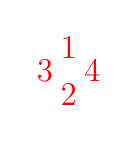
\begin{tikzpicture}[scale=0.3, baseline=-1mm, thick]
                  \draw[color=red] (10mm,0) node {\large 4};
                  \draw[color=red] (-10mm,0) node {\large 3};
                  \draw[color=red] (0,10mm) node {\large 1};
                  \draw[color=red] (0,-10mm) node {\large 2};
            \end{tikzpicture}
            \vspace*{-7pt}
      \item Kreśli znak krzyża nad wodą na \textit{Benedico te}
      \item Po zmianie głosu na \textit{recto tono} na słowa \textit{tu benignus
                  aspira} trzy razy dmucha do wody na kształt krzyża
      \item W tym czasie ceremoniarz podaje Paschał
      \item Na słowa \textit{Descendad in hanc} trzy razy wkłada Paschał do wody
            i śpiewa \footnote{Wkłada Paschał coraz głębiej}
      \item \ii~ trzy razy dmucha do wody w kształcie litery
            \textcolor{red}{\raisebox{-1mm}{\Large ${\Psi}$}} i kontynuuje
            \textit{Totamque ... effectu}
      \item Wyciągamy Paschał z wody i kończymy święcenie wody (\textit{... per
                  ignem.})
      \item Po wyjęciu paschału nabiera się wody do pokropienia
      \item Następnie \cc1 przynosi do chrzcielnicy tackę z olejami świętymi i
            wręcza \ii~ (z pocałunkiem) odpowiednie ampułki. \ii, wypowiadając
            słowa przepisane w księdze po kolei:
            \begin{itemize}
                  \item wlewa olej katechumenów
                  \item wlewa krzyżmo
                  \item wlewa oba
            \end{itemize}
      \item Następnie miesza wodę ręką lub przy pomocy łyżeczki
      \item Później myje i wyciera ręce \footnote{W razie potrzeby wykorzystuje
                  sól, watę i miękisz chleba, które później należy spalić. Wodę
                  z tej ablucji wlewa
                  się do sacrarium.}
\end{enumerate}

\subsection{Bierzmowanie}
\label{sec:bierz}
\begin{itemize}
      \item księgę z modlitwami trzyma \cc1, a \cc2 podtrzymuje kapę jeśli
            trzeba; \aa1 i \aa2 stoją z boku przy kredencji
      \item \ii~ odmawia modlitwę zwracając się do kandydatów \textit{Spiritus
                  Sanctus superveniat\dots}
      \item \ii~ czyni znak Krzyża Świetego mówiąc \textit{Adjutorium
                  nostrum...} a następnie kontynuowany jest krótki dialog
      \item \ii~ wyciąga ręce nad przystępującymi do bierzmowania i mówi
            \textit{Oremus. Omnipotens sempiterne Deus,...}
      \item przystępujący do sakramentu klęka przed \ii. Świadek kładzie rękę na
            prawym ramieniu bierzmowanego.
      \item \aa1 podchodzi do \ii~ z Krzyżmem Świętem
      \item \ii~ kładzie prawą rękę na głowie bierzmowanego i palcem umoczonym w
            Krzyżmie Świętym robi znak krzyż a na czole, mówiąc \textit{Signo te
                  signo...}
      \item \ii~ uderza lekko w policzek bierzmowanego, mówiąc \textit{Pax tecum}
      \item kandydat wraca na swoje wcześniejsze miejsce i stoi
      \item \aa1 odbiera Krzyżmo, a \aa2 podchodzi z czymś do wytarcia palców
            \footnote{najpewniej wata}; później wracają do kredencji
      \item gdy \ii~ namaści wszystkich kandydatów, śpiewa się antyfonę
            \textit{Confirma hoc, Deus\dots}
      \item powtarza się antyfonę, a następnie \ii~ zwrócony do ołtarza śpiewa
            \textit{Ostende nobis, Domine,...}, a następnie \textit{Oremus.
                  Deus, qui Apostolis tuis\dots}
      \item \ii~ mówi \textit{Ecce sic benedicetur omnis homo, qui timet Dominum}
      \item na końcu \ii~ błogosławi bierzmowanych
            \textit{Bene} + \textit{dicat vos Dominus ex Sion...}
\end{itemize}

\color{red}

\section{Uwagi}
\begin{itemize}
      \item można zrobić jakieś święcenie ognia przed proroctwami tak aby ludzie
            oświetlali kościół i mieć jakąś namiastkę Wigilii Paschalnej
      \item na poświęcenie wody ludzie \textbf{muszą mieć zapalne świece}
      \item zapytać księdza czy będzie aspersja (czy to humanitarne?)
      \item ziomek do chrztu musi siedzieć za kratą aż do ochrzczenia -- trzeba
            mu przygotować jakieś krzesło i klęcznik
      \item na chrzest dorosłego ksiądz ubiera kapę (patrz Nowowiejski)
\end{itemize}

% \section{Procesja do Bożego Grobu}

\begin{itemize}
	\item \tt1 i \tt2 wychodzą z kadzielnicami, \oo~ - z ombrelino, \ding{63}
	      staje z krzyżem procesyjnym u wejścia do prezbiterium
	\item ministranci zapalają swoje świece
	\item \aa1 przynosi na ołtarz monstrancje i przejrzysty welon do niej
	\item \ii~ wraz z \cc1 i \cc2 udaje się do stopni ołtarza i sam wchodzi na
	      górę
	\item po wystawieniu Najświętszego Sakramentu \ii~ schodzi po stopniach,
	      zasypuje kadzidło i okadza N. S.
	\item po okadzeniu \cc2 nakłada \ii~ welon naramienny i wraca na miejsce
	\item \aa1 i \aa2 z akolitkami (wziętymi z kredensji) dołączają do \ding{63}
	\item \cc1 i \cc2 biorą kołatki
	\item gdy \ii~ bierze monstrancję, formuje się procesja w kolejności:

	      \begin{enumerate}\centering
		      \item[] (stopnie ołtarza)
		      \item[] \cc2~~~\ii~~~~\oo~~~~\cc1
		      \item[] \tt1~~~\tt2
		      \item[] chór ze świeczkami (parami)
		      \item[] \aa2~~~\ding{63}~~~\aa1
	      \end{enumerate}

	      \newpage

	      \begin{figure}[h]
		      \centering
		      \includegraphics[scale=0.6]{Piatek/Procesja1.pdf}
	      \end{figure}

	\item po dokonaniu wystawienia w Bożym Grobie następuje zasypanie i
	      okadzenie oraz krótka adoracja

	      \begin{figure}[h]
		      \centering
		      \includegraphics[scale=0.7]{Piatek/Procesja2.pdf}
	      \end{figure}

	\item procesja udaje się do zakrysti
\end{itemize}



\end{document}
